\documentclass[a4paper,12pt]{report}
\usepackage[utf8]{inputenc}
\usepackage{amsmath}
\usepackage{graphicx}
\usepackage{listings}
\usepackage{tikz}

\usepackage{color}
\usetikzlibrary{arrows,automata}
\definecolor{pythonred}{rgb}{0.6,0,0} % for strings
\definecolor{pythongreen}{rgb}{0.25,0.5,0.35} % comments
\definecolor{pythonpurple}{rgb}{0.5,0,0.35} % keywords
	\definecolor{pythondocblue}{rgb}{0.25,0.35,0.75} % javadoc
	\renewcommand{\thechapter}{}
	\renewcommand{\chaptername}{}
	\lstset{language=python,
	basicstyle=\ttfamily,
	keywordstyle=\color{pythonpurple}\bfseries,
	stringstyle=\color{pythonred},
	commentstyle=\color{pythongreen},
	morecomment=[s][\color{pythondocblue}]{/**}{*/},
	numbers=left,
	numberstyle=\tiny\color{black},
        stepnumber=2,
	numbersep=10pt,
	tabsize=4,
	showspaces=false,
	showstringspaces=false}

% Title Page

  \title{\bfseries\huge \textcolor{purple}{EEP701 Digital System Lab} \\{\textcolor{brown}{Assignment8-Interface a Keyboard with an FPGA spartan 3 kit}}}
\author{\bfseries\large\textcolor{black} {Abhishek Ranjan}\\ {\textcolor{black}{2013EET2365}}\\{\bfseries\large\textcolor{black}{Harshit Gupta}} \\{\textcolor{black}{2013EET2369}}\\

\includegraphics[width=3cm,height=3.4cm]{./iit.png}\\\noindent Computer Technology\\
\noindent Department Of Electrical Engineering}
% iit.png: 282x282 pixel, 72dpi, 9.95x9.95 cm, bb=0 0 282 282



\begin{document}
\maketitle
\tableofcontents




\begin{center}
\chapter{\textcolor{blue}{PROBLEM STATEMENT}}
\end{center}
\noindent  Interfacing a keyboard with an FPGA Spartan 3 kit through a PS2 port and display the inputs in the 7-segment
display. Your objective in this assignment
 to interface a  keyboard with Spartan board and display the typed characters on a 7
segment LED display. The LED display supports 4 characters at once.
You have to write an interpreter in VHDL to interpret the code received from keyboard into a
character. The interpreter in this case should work like an FSM. There is a unique scan code
generated for each character typed from keyboard. Interpretation should be done for following
keys:
 \begin{itemize} \item Printable characters: alphabets and numerals
 \item  Control keys: CAPS LOCK, SPACEBAR and BACKSPACE
 \end{itemize}

 
 \noindent Display of characters on LED display should be done in following way:
\begin{itemize} \item Keystrokes : CAPSLOCK A CAPSLOCK B C D
\\Display : dcbA
\item Keystrokes: A CAPSLOCK H SPACE 3
\\Display: 3   H a
\item Keystrokes: 1 2 3 BACKSPACE 4 5
\\Display: 5 4 2 1
\end{itemize}

\begin{center}
\chapter{\textcolor{blue}{ABSTRACT}}
\end{center}
\noindent This report is on interfacing a keyboard with a Spartan kit usnig VHDL.
The Objective of this Assignment is to understand the woking of a keyboard and th
interfacing to different devices with a kit.The interfaceing is done through a PS2 
port that are available on board a Spartan 3 kit.Generally all keyboards have a PS2
interface.We have to show the character the characters that are input through the keyboard.
We store the inputs done afer each keystore and display the latest of them in the 
7 segment display that is available on the board.We also have to implemant the shift and caps lock
entries and give the corresponding outputs to the display.Also ``backspace'' is also implemented.
\begin{center}
\chapter{\textcolor{blue}{INTRODUCTION}}
\end{center}
\noindent VHDL (VHSIC Hardware Description Language) is a hardware description language used in 
electronic design automation to describe digital and mixed-signal systems such as field-programmable
gate arrays and integrated circuits. VHDL can also be used as a general purpose parallel programming language.\\

  The idea of being able to simulate the ASICs from the information in this documentation was so obviously attractive 
that logic simulators were developed that could read the VHDL files. The next step was the development of logic 
synthesis tools that read the VHDL, and output a definition of the physical implementation of the circuit.\\

Xilinx ISE (Integrated Software Environment) is a software tool produced by Xilinx for synthesis and 
analysis of HDL designs, enabling the developer to synthesize ("compile") their designs, perform timing
analysis, examine RTL diagrams, simulate a design's reaction to different stimuli, and configure the target
device with the programmer.\\

This report is on interfacing a keyboard with a Spartan kit usnig VHDL.
The Objective of this Assignment is to understand the woking of a keyboard and th
interfacing to different devices with a kit.The interfaceing is done through a PS2 
port that are available on board a Spartan 3 kit.Generally all keyboards have a PS2
interface.We have to show the character the characters that are input through the keyboard.
We store the inputs done afer each keystore and display the latest of them in the 
7 segment display that is available on the board.We also have to implemant the shift and caps lock
entries and give the corresponding outputs to the display.Also ``backspace'' is also implemented.
 
\begin{center}
\chapter{\textcolor{blue}{SPECIFICATIONS AND ASSUMPTIONS}}
\end{center}
\section*{Specifications and Assumptions}

\begin{itemize}
\item \noindent Total of 100 Characters can be stored on the chip which could be dispalyed on the display
\item\noindent Left Shift an Right Shift work
\item\noindent Caps lock is also assimilated
\item \noindent Backspace deletes the last character from the input stream
\item The keys which cannot be displayed would be bypassed and not be shown in the display
\end{itemize}

\begin{center}
\chapter{\textcolor{blue}{LOGIC USED/METHODOLOGY}}
\end{center} 
\section*{Getting the key code}
\noindent We use FSM for getting the inputs.A clock and code comes from the keyboard when a key is pressed.It s starts with a start bit .
This is fallowed by an 8 bit code of the key that is pressed.This code is the keycode which supplies the information of what key is pressed.
The next bit is parity bit and then a stop bit is generated.When a key is released, a similar code is sent which is of 2 bytes.

\section*{Getting the seven segment display code}
\noindent We have to assign the code for displaying the characters in the seven segment display by assigning the given codes
to each symbol.We have created allokup table for that.If shift is pressed or caps lock is on then a seperate lookup table 
is reffered to.This is the code which is passed in to the display unit to display in the seven segment display.This code is 
pushed into a input buffer which stores all the input characters sent till that time.If backspace is pressed , then we delete
the last code from the input stream.\\

\section*{Displaying }
\noindent There are 4 display units in the Spartan kit.We can display 4 characters at the same time.The display on the 4
units are done in a time division basis.We have seperate enable signal for each of the 4 units.and the same control signal is 
sent to them.so we time multiplex the control signal and change the control signal in synchronyzation with that.We
are able to display 1 characters from the input stream at one time.But we change these control signals  so frequently that 
to human eye it appears to be displaying simultaneously.This is how displaying is done \\


\begin{center}
\chapter{\textcolor{blue}{FLOWCHART}}
\begin{center}
 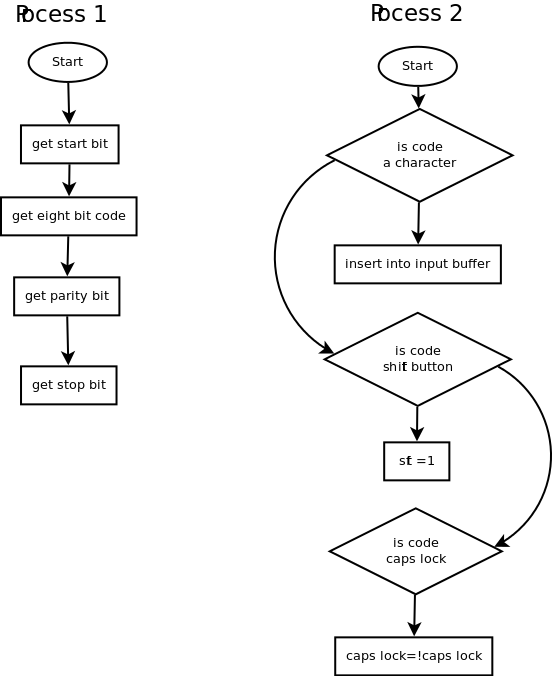
\includegraphics[scale=0.5]{./flowchart.png}
 % Xlinx6_flowchat.png: 1097x637 pixel, 72dpi, 38.70x22.47 cm, bb=0 0 1097 637
\end{center}

\end{center}

\begin{center}
\chapter{\textcolor{blue}{OBSERVATIONS}}
\begin{center}
 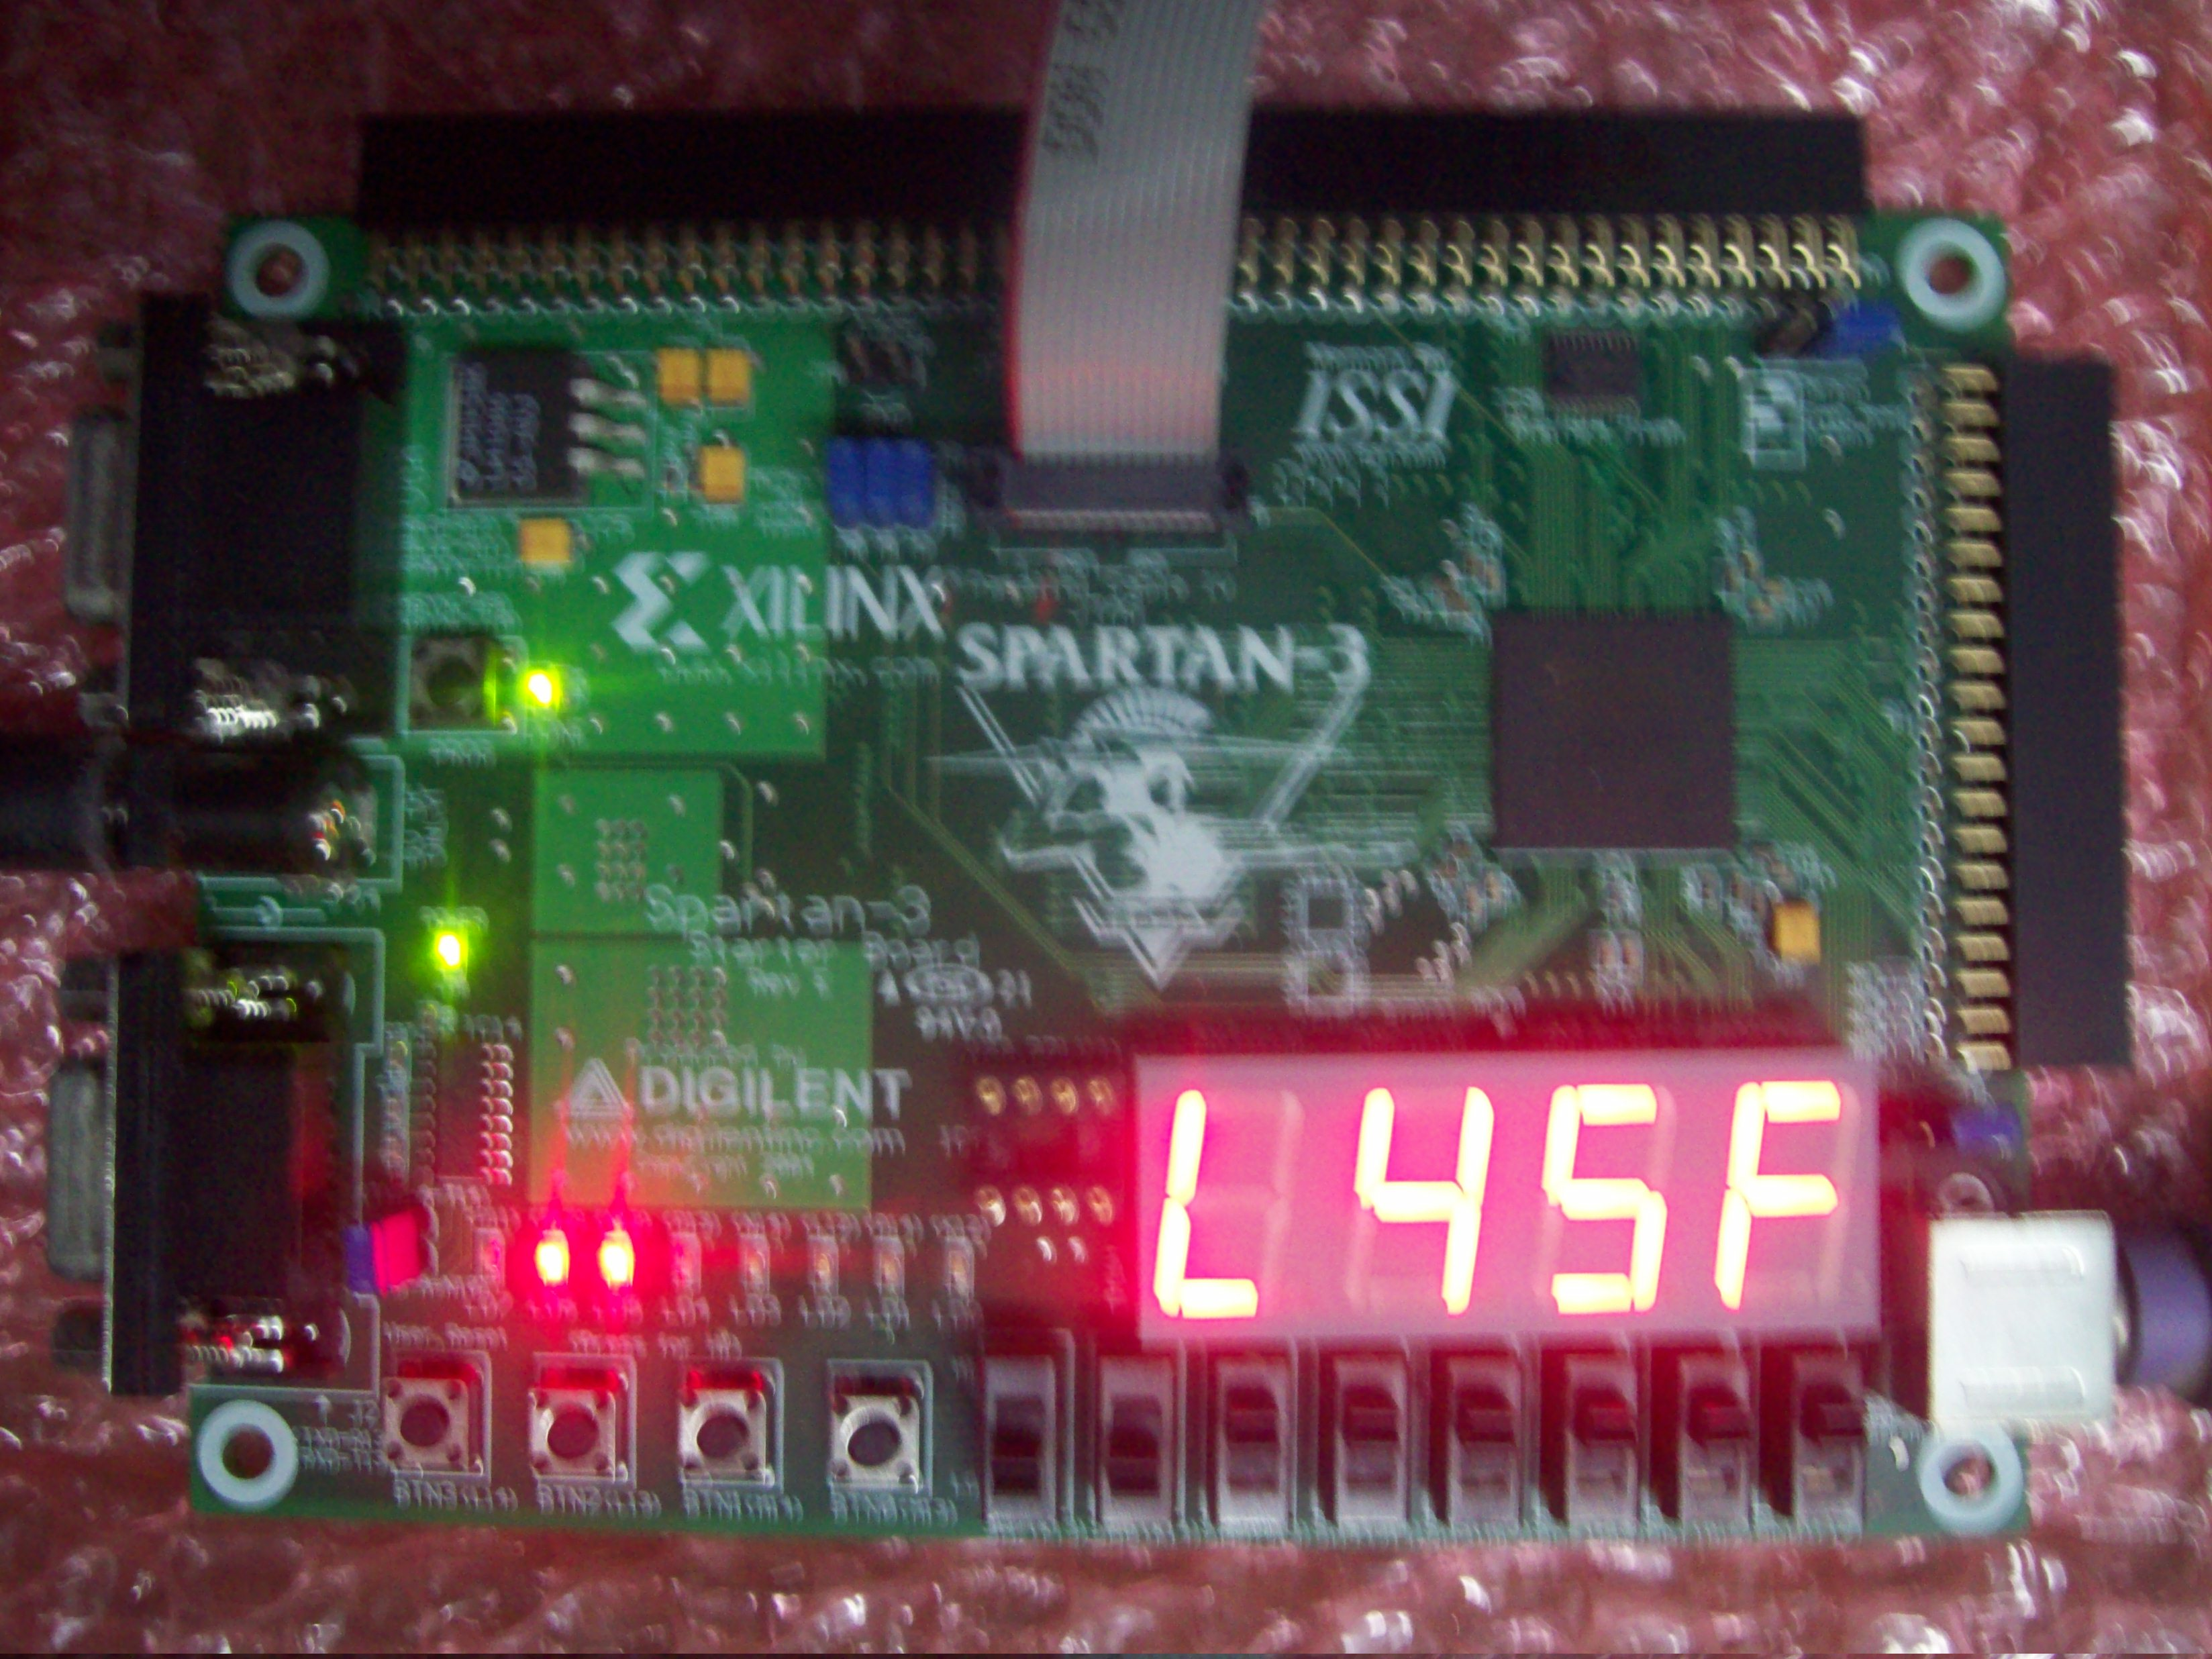
\includegraphics[scale=0.1]{./working_1.JPG}
 % Capture.PNG: 890x270 pixel, 96dpi, 23.55x7.14 cm, bb=0 0 668 203
\end{center}

\end{center}






\begin{center}
\chapter{\textcolor{blue}{RESULTS AND CONCLUSIONS}}\end{center}

\noindent The keyboard interface with Spartan 3 kit was sucessfully designed and implemented on board.We got to learn 
how to interface devices and to take signals from various kinds of ports,how to handshake,etc.Also we got a chance to
implement it on board and thus gave us exposure to designing  ASIC chips.

\end{document}  